\section{Funktionenfolgen und deren Konvergenz}
\subsection{Funktionenfolgen und deren Konvergenz}
Ist $ \Omega \subset \R  $ nichtleer und für jedes $ n \in \N  $ eine Funktion $ f_n : \Omega \to \R  $ definiert, so nennen wir $ (f_n) $ eine Funktionenfolge

\begin{subexample}
	Sei für $ n \in \N \quad f_n : \Omega \to \R , x \mapsto x^n $. z.B.
	\begin{enumerate}[label=\arabic*.]
		\item $ f_1: \Omega \to \R , x \mapsto x $ 
		\item $ f_2: \Omega \to \R , x \to x^2 $
		\item usw.
	\end{enumerate}
\end{subexample}

\begin{subdefinition}[Punktweise Konvergenz]
	Sei $ \Omega \subset \R  $ nichtleer und $ f, f_1, f_2, \dotsc: \Omega \to \R  $.\\
	Wir sagen $ (f_n) $ \textbf{konvergiert punktweise gegen} $ f $, falls $ \forall x \in R $ die Folge $ (f_n(x)) $ gegen $ f(x) $ konvergiert.\\
	Gibt es ein $ f:\Omega\to \R  $, so dass $ (f_n) $ punktweise gegen $ f $ konvergiert, so nennen wir $ (f_n) $ \textbf{punktweise konvergent}.\\
	Wir nennen dann $ f $ \textbf{Grenzfunktion} von $ (f_n) $.\\
	Das bedeutet:
	\[
		\forall x \in \Omega: \forall \varepsilon > 0 : \exists N \in \N : \forall n \geq N: |f_n(x) - f(x) | < \varepsilon 
	\]
\end{subdefinition}
\textbf{Beachte:} Bei punktweiser Konvergenz sehen wir uns also für jedes $ x \in \Omega $ an, gegen welchen Wert $ f_n(x) $ konvergiert. Definieren wir dann $ f(x) \coloneqq \lim_{n \to \infty} f_n(x) $, so ist $ f:\Omega \ni x \to f(x) $ der punktweise Limes der Funktionenfolge $ (f_n) $
\begin{subexample}
	Sei $ \Omega = [0, 1] $. Wir betrachten $ f_n: \Omega \to \R  $ mit $ f_n(x) = x^n, x \in [0, 1] $.\\
	Ist $ x \in [0, 1) $, so $ \lim_{n \to \infty} f_n(x) = 0 $. Hingegen $ \lim_{n \to \infty} f_n(x) = 1 $ für $ x = 1 $.
	Also konvergiert $ (f_n) $ punktweise gegen
	\[
		f: \Omega \to \R \text{ mit } f(x) \coloneqq \begin{cases}
			0 & \text{für } 0\leq x<1\\
			1 & \text{für } x = 1
		\end{cases}
	\]
\end{subexample}
\begin{figure}[!ht]
	\centering
	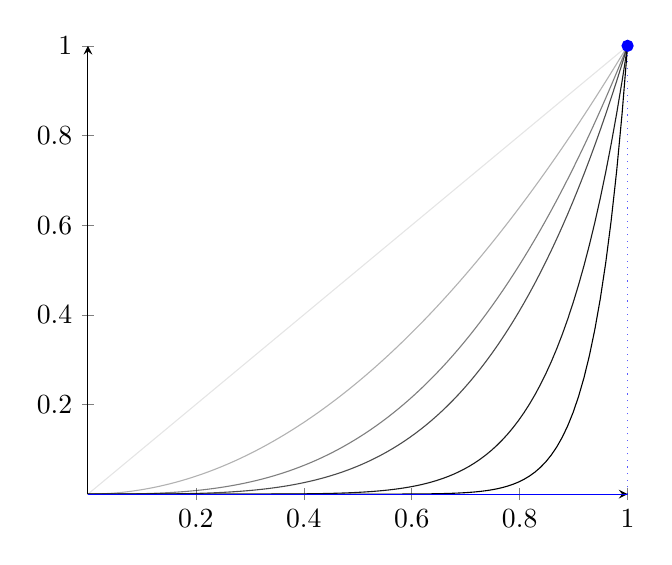
\begin{tikzpicture}
		\begin{axis}[
			xmin= 0, xmax= 1,
			ymin= 0, ymax = 1,
			axis lines = middle,
		]
			\addplot[domain=0:1, samples=100, opacity = 0.1]{x};
			\addplot[domain=0:1, samples=100, opacity = 0.3]{x^2};
			\addplot[domain=0:1, samples=100, opacity = 0.5]{x^3};
			\addplot[domain=0:1, samples=100, opacity = 0.7]{x^4};
			\addplot[domain=0:1, samples=100, opacity = 0.9]{x^8};
			\addplot[domain=0:1, samples=100, opacity = 1.0]{x^16};
			\addplot[domain=0:1, samples=100, color = blue]{0};
			\addplot[color = blue, mark = *, only marks] coordinates{(1,1)};
			\draw[dotted, color = blue] (axis cs:1,0) --(axis cs:1,1);
		\end{axis}
	\end{tikzpicture}
	\caption{Definition 8.1.2}
	\label{Definition8.1.2}
\end{figure}

\begin{subdefinition}[Gleichmäßige Konvergenz]
	Sei $ \Omega \subset \R  $ nichtleer und $ f, f_1, f_2, \dotsc : \Omega \to \R  $.
	Wir sagen $ (f_n) $ \textcolor{gadse-dark-green}{konvergiert gleichmäßig gegen} f, falls für jedes $ \varepsilon > 0 $ ein $ N \in \N  $ existiert, sodass $ |f(x) - f_n(x)| < \varepsilon  $ f.a. $ x \in \Omega $ und alle $ n \geq N $ gilt.\\
	Das bedeutet:
	\[
		\forall \varepsilon > 0: \exists N \in \N \forall n \geq N : \forall x \in \Omega: |f_n(x) - f(x)| < \varepsilon .
	\]
\end{subdefinition}

\begin{sublemma}
	Sei $ \Omega \subset \R  $ nichtleer und $ f, f_1, f_2, \dotsc : \Omega \to \R  $ so, dass $ (f_n) $ gleichmäßig gegen $ f $ konvergiert.
	Dann konvergiert $ (f_n) $ auch punktweise gegen $ f $.
\end{sublemma}

\begin{subexample}
	Die Folge aus Beispiel \ref{8.1.3} konvergiert nicht gleichmäßig.\\
	Sei $ 1 > \varepsilon > 0, N \in \N  $ beliebig. Setzte $ x \coloneqq \sqrt[n]{\varepsilon }   $. Dann ist $ x_0 \in (0, 1) $ und $ f_n(x_0) = \varepsilon  $, d.h. $ |f_n(x_0) - f(x_0)| = |f_n(x_0)| = \varepsilon \geq \varepsilon  $
\end{subexample}

\begin{subtheorem}
	Sei $ \Omega \subset \R  $ nichtleer und $ f_1, f_2, \dotsc : \Omega \to \R  $ stetige Funktionen.
	Konvergiert $ (f_n) $ gleichmäßig gegen $ f: \Omega \to \R  $, so ist $ f $ stetig.
\end{subtheorem}

\begin{subproof*}[Theorem \ref{8.1.7}]
	Sei $ x_0 \in \Omega $ und $ \varepsilon > 0 $ beliebeig. Dann finden wir wegen glm. Konv. ein $ N \in \N $
	mit $ |f_n(x) - f(x)| < \frac{ \varepsilon  }{ 2 }  $ für alle $ x \in \Omega $. Nun ist $ f_N $ stetig, und daher gibt es ein $ \delta > 0 $ so, dass $ \left| x_0 - x \right| < \delta $ die Ungleichung $ \left| f_N(x_0) - f_N(x) \right| < \frac{\varepsilon}{ 3 }  $ nach sich zieht. Damit folgt
	\begin{align*}
		\left| f(x) - f(x_0) \right| &\leq \left| f(x) - f_N(x) \right| + \left| f_N(x) - f_N(x_0) \right| + \left| f_N(x_0) - f(x_0) \right| \\
		~&< \frac{ \varepsilon }{ 3 } + \frac{ \varepsilon }{ 3 } + \frac{ \varepsilon }{ 3 } = \varepsilon 
	\end{align*}
	Damit haben wir gezeit, dass $ f $ stetig ist.
\end{subproof*}

$ (f_n), f_n : \Omega \to \R  $ Funktion.\\
können wir Konzepte der Folgen auch auf Funktionenfolgen anwenden?\\
$ (a_n) \subset \R \mapsto (f_n : \Omega \ni x \mapsto a_n) $
$ f, f_1, f_2, \dotsc : \Omega \to \R , f_n \to  f  $ punktweise Konvergent $ \iff \forall x \in \Omega : f(x) = \lim_{n \to \infty} f_n(x) $\\
Sind alle $ f_n $'s stetig, so nicht unbedingt $ f $!\\
\textbf{Verschärfung:} $ f_n \to f $ \textbf{gleichmäßig}, falls $ \forall \varepsilon > 0 : \exists N \in \N : \forall n \geq N : \forall x \in \Omega : | f_n(x) - f(x) | < \varepsilon  $.
\begingroup
\color{green}
\textbf{Punktweise Konvergenz}:
$ \forall x \in \Omega : \forall \varepsilon > 0 : \exists N \in \N  : \forall n \geq N : | f_n(x) - f(x) | \varepsilon  $ 
\endgroup

\begin{itemize}
	\item Bei gleichmäßiger Konvergenz $ f_n \to f: $ Alle $ f_n $'s stetig $ \implies f $ stetig.
\end{itemize}

\subsection{Normierte Vektorräume stetiger Funktionen}
\textbf{In Vektorräumen:}
\begin{itemize}
	\item Addition möglich
	\item Multiplikation mit Skalaren möglich
	\item Nullvektor ($ \hat{=} $ neutrales Element der Addition)
\end{itemize}
$ \Omega \in \R  $ nichtleer, dann bilden die stetigen Funktionen auf $ f: \Omega \to \R  $ einen \textbf{Vektorraum} (über $ \R  $), den wir \fbox{$ C(\Omega) $} nennen. Für $ \lambda, \mu \in \R , f,g \in C(\Omega): \lambda f + \mu g : \Omega \ni x \mapsto \lambda f(x) + \mu g(x) \in \R  $.\\
Der Nullvektor ist hier die Nullfunktion, $ \mathbf{0} : \Omega \ni x \mapsto 0 \in \R  $.


Wir wollen an dieser Stelle einen systematischeren Blick auf die im letzten Abschnitt eingeführte gleichmäßige Konvergenz von Funktionenfolgen entwickeln. Hierzu sei $ \Omega \subset  \R  $ nichtleer. Setzen wir $ \mathbf{0}: \Omega \ni x \to 0 $ sowie für $ \lambda, \mu \in \R  $ und $ f,g:\Omega \to \R  $ 
\[
	(\lambda f + \mu g): \Omega \ni x \to \lambda f(x) + \mu g(x) \in \R ,
\]
so erhalten die stetigen Funktionen eine \textbf{Vektorraumstruktur}. Dies ist erst einmal eine rein algebraische Struktur. Nun ist eine naheliegende Frage, wie wir \textbf{Längen} von Vektoren messen können. Dies soll den folgenden vier Prinzipien genügen:
\begin{enumerate}[label=(P\arabic*)]
	\item Längen von Vektoren sind stets nichtnegativ und endlich. \textit{Dies ist sonnvoll:} Wir würden zum Beispiel niemals sagen, ein Stab sei $ \qty{ -3 }{ \metre }  $ lang.
	\item Hat ein Objekt die Länge Null, so ist dies notwendigerweise der Nullvektor. \textit{Dies ist sinnvoll:} Hat ein Objekt Länge Null, so hat es keine Ausdehnung und ist damit der Nullvektor.
	\item Strecken wir ein Objekt um den Faktor $ \lambda \geq 0 $, so hat das gestreckte Objekt die $ \lambda $-fache Länge des urspprünclichen Objekts. Eine Streckung mit einem Faktor $ \lambda < 0 $ bedeutet, dass wir die Ausrichtung des ursprünclichen Objekts umkehren und dann mit dem Faktor $ \left| \lambda \right| $ strecken. Damit sollte $ \left\| \lambda x \right\| = \left| \lambda \right| \left\| x \right\|  $ gelten.
	\item Die Dreiecksungleichung besagt, dass wir einen Umweg machen, wenn wir nicht direkt von einem Punkt $ x_1 $ zu einem anderen Punkt $ x_3 $ laufen, sondern erst von $ x_1 $ zu $ x_2 $ und dann von $ x_2 $ zu $ x_3 $ laufen
\end{enumerate}

\textbf{Ziel:} Ordne Funktionen eine ``Länge'' zu.
\begin{subdefinition}
	Sei $ X $ ein $ \R  $-Vektorraum. Eine Abbildung $ \left\| \cdot  \right\|: \to \R _{\geq 0}  $ heißt \textbf{Norm} (Längenfunktion), falls:
	\begin{enumerate}[label=(\roman*)]
		\item $ \left\| x \right\| = 0 \iff x = \mathbf{0} $ (also $ x $ der Nullvektor in $ X $ ist).
		\item $ \forall \lambda \in \R : \forall x \in X : \left\| \lambda x \right\| = \left| \lambda \right| \left\| x \right\| $
		\item $ \forall x,y \in X: \left\| x + y \right\| \leq \left\| x \right\| + \left\| y \right\| $. (Dreiecksungleichung)
	\end{enumerate}
	Das Tupel $ \left( X, \left\| \cdot  \right\| \right)  $ heißt dann \textbf{normierter Vektorraum}.
\end{subdefinition}

\begin{subdefinition}
	Sei $ \left( X, \left\| \cdot  \right\|  \right)  $ ein normierter Vektorraum sowie $ x, x_1, x_2, \dotsc \in X $. Wir sagen, dass $ \left( x_n \right)  $ (bezüglich $ \left\| \cdot  \right\|  $) gegen $ x $ \textbf{konvergiert}, falls
	\[
		\lim_{n \to \infty} \left\| x_n - x \right\| = 0,
	\]
	d.h. für jedes $ \varepsilon > 0 $ existiert ein $ N \in \N  $ so, dass $ \left\| x_n - x \right\| < \varepsilon  $ für alle $ n \geq N $ gilt.
\end{subdefinition}

Das für uns wichtigste Besipiel ist die \textbf{Supremumsnorm:}
\begin{subexample}[Supremumsnorm]
	$ C_b(\Omega) \coloneqq  \left\{ f: \Omega \to \R : f \text{stetig und beschränkt}  \right\}  $. ($ f \text{ beschränkt } \iff \exists M \geq  0 \forall  x \in  \Omega : | f(x) | \leq M $). Dies ist auch ein Vektorraum, und es definiert
	\[
		\left\| f \right\|_{\infty, \Omega} \coloneqq \sup_{x \in \Omega} | f(x) |, f \in C_b(\Omega) 
	\]
	 eine \textbf{Norm darauf}.
	\begingroup
	\color{blue}
	(Auf $ C(\Omega) $ \textbf{nicht:} z.B. $ \Omega = (0, 1), f(x) \coloneqq \frac{ 1 }{ x }  $, dann $ \left\| f \right\|_{\infty, \Omega} \nless \infty ) $
	\endgroup
\end{subexample}

$ \left\| \cdot  \right\|_{\infty, \Omega} $ ``Supremumsnorm'' ( $ \widehat{=} $ Länge/Größe von Funktion)

\begin{enumerate}[label=(\roman*)]
	\item[(0)] $ \left\| \cdot  \right\|_{\infty, \Omega} : C_b(\Omega) \to  \R_{\geq 0} $. (Hier geht ein: $ f \in C_b(\Omega) $ beschränkt)
\item $ f \in C_b(\Omega) \wedge \underbrace{\left\| f \right\|}_{\infty, \Omega} = 0 $, zu zeigen \fbox{$ f = 0 $}
		\[
			\sup_{x \in \Omega} | f(x) | = 0 \implies (\forall x \in  \Omega : f(x) = 0) \implies f = 0.
		\]
		und $ \left\| \mathbf{0} \right\|_{\infty, \Omega} = \sup_{x \in \Omega} 0 = 0 $.
	\item $ \lambda \in \R , f \in C_b(\Omega) $, so ist $ \forall x \in \Omega : | \lambda f(x) | =  $ 
		\begin{align*}
			~&= |\lambda| |f(x)| \implies  \left\| \lambda f \right\|_{\infty, \Omega} \\
			~&= \sup_{x\in \Omega} | \lambda f (x) | \\
			~&= \sup_{x \in \Omega} |\lambda| |f(x)| \\
			~&= |\lambda| \sup_{x \in \Omega} |f(x)| \\
			~&= |\lambda| \left\| f \right\|_{\infty, \Omega}. \\
		\end{align*}
	\item $ f, g \in  C_b(\R ) $.
		Dann
		\[
			\forall x \in \Omega: | f(x) + g(x) |
			\leq \underbrace{|f(x)|}_{\leq \left\| f \right\|_{\infty, \Omega}}
				+ \underbrace{g(x)}_{\leq \left\| g \right\|_{\infty, \Omega}}
			\leq \left\| f \right\|_{\infty, \Omega}
				+ \left\| g \right\|_{\infty, \Omega}.
		\]
		Supremum in $ x $
\end{enumerate}

\begin{itemize}
	\item Beachte: $ (\R , \left\| \cdot  \right\|)  $ ist auch normierter Raum.
\end{itemize}
\textbf{Konvergenz:} $ \forall \varepsilon > 0 : \exists N \in  \N  : \forall n \geq N : \left\| x_n - x \right\| < \varepsilon  $ 

\begin{subdefinition}
	Sei $ (X, \left\| \cdot  \right\| ) $ normierter Vektorraum, sowie $ x, x_1, x_2, \dotsc \in X $. Wir sagen, $ (x_n) $ \textbf{konvergiert} bezüglich $ \left\| \cdot  \right\|  $ gegen $ x $, falls $ \forall \varepsilon > 0: \exists N \in \N : \forall n \geq N : \left\| x_n - x  \right\| < \varepsilon $
\end{subdefinition}

\begin{subproposition}
	Sei $ \Omega \subset \R  $ nichtleer, $ f, f_1, \dotsc \in C_b(\Omega) $.
	Dann konvergiert $ (f_n) $ genau dann gleichmäßig gegen $ f $, wenn $ (f_n) $ bezüglich $ \left\| \cdot  \right\|_{\infty, \Omega} $ gegen $ f $ konvergiert.
	{\color{green} $ \iff \lim_{n \to \infty} \left\| f_n - f \right\|_{\infty, \Omega} = 0 $}
	\begin{description}
		\item[``$ \implies  $'']
			\begin{align*}
				&\forall \varepsilon > 0: \exists N \in \N  : \forall  n \geq  N : ( \forall x \in \Omega: |f_n(x) - f(x)| < \varepsilon )\\
				&\forall \varepsilon > 0: \exists N \in \N  : \forall  n \geq  N : \left( \sup_{x \in \Omega}: |f_n(x) - f(x)| \leq  \varepsilon \right)\\
				&(\forall \varepsilon > 0: \exists N \in \N  : \forall  n \geq  N : | |f_n(x) - f(x)| |_{\infty, \Omega} \leq  \varepsilon ) \implies  f_n \to f, \left\| \cdot  \right\|_{\infty, \Omega} \qed
			\end{align*}
	\end{description}
\end{subproposition}

\begin{subexample}
	$ f_n : \R  \ni x \mapsto \frac{ 1 }{ n(1 + x^2) } \in \R  $.\\
	\textbf{Punktweise Konvergenz} $ f_n(x) = \frac{ 1 }{ n } \cdot \left(  \frac{ 1 }{ 1 + x^2 } \right) \to 0 $.
	Also $ f_n \to 0 $ punktweise konvergent.\\
	\textbf{Gleichmäßig Konvergent} bedeutet nach Proposition \ref{8.2.4}:
	\begin{align*}
		\lim_{n \to \infty} \sup_{x \in \R } |f_n(x) - \underbrace{f(x)}_{0}| &= \left( \lim_{n \to \infty} \left\| f_n - f \right\|_{\infty, \omega} \right) \\
		~&= 0 \\
	\end{align*}
	\textbf{Hier:}
	\[
		\sup_{x \in \R } |f_n(x) - \underbrace{f(x)}_{=0} = \frac{ 1 }{ n } \underbrace{\sup_{x \in \R} \frac{ 1 }{ 1+x^2 }  }_{=1} = \frac{ 1 }{ n } ,
	\]
	also 
	\[
		\lim_{n \to \infty} \left\| f_n - f \right\|_{\infty, \Omega} = \lim_{n \to \infty} \frac{ 1 }{ n } = 0.
	\]
	gleichmäßige Konvergenz
\end{subexample}

\begin{subexample}
	\[
		f_n : [0, 1] \ni x \mapsto x^n \in \R,
	\]
	so $ f_n \to f $ punktweise konvergent mit
	\[
		f(x) = \begin{cases}
			0, & x \in [0, 1),\\
			1, & x = 1
		\end{cases}.
	\]
	Haben 
	\[
		\sup_{x \in [0, 1]} | f_n(x) - f(x)| = \sup_{x \in [0, 1)} | x^n | \overset{n\to \infty}{\nrightarrow} 0
	\]
	
\end{subexample}

\subsection{Potenzreihen}
\[ a_0 + a_1x + a_2 x^2 + \dotsc + a_N x^N = \sum_{n=0}^{N} a_nx^n \]
\begin{subdefinition}
	Sei $ (a_n)_{n \in \N_0} \subset \R \wedge x_0 \in \R  $. Dann heißt der \textbf{formale Ausdruck}  
	\[
		f(x) = \sum_{n=0}^{\infty} a_n(x - x_0)^n
	\]
	\textbf{formale Potenzreihe} mit \textbf{Entwicklungspunkt} $ x_0 $.\\
	Die \textbf{Konvergenzmenge} von $ f $ ist
	\[
		D_f \coloneqq \left\{ x \in \R : \sum_{n=0}^{\infty} a_n(x-x_0)^n \text{ konv.}  \right\} 
	\]
	Wir nennen dann $ f: D_f \to \R  $ die durch die Potenzreihe \textbf{dargestellte Funktion} (kurz auch \textbf{Potenzreihe})
\end{subdefinition}

\begin{subexample}
	\[
		f(x) = \sum_{n=0}^{\infty} x^n.
	\]
	Dies konvergiert genau dann wenn $ |x| < 1 $.\\
	Geometrische Reihe: $ f(x) = \frac{ 1 }{ 1 - x } = \underbrace{\underbrace{1 + x} + x^2 + \dotsc} $
\end{subexample}

\begin{subtheorem}[Weierstraßsches Konvergenzkriterium]
	Sei $ A \subseteq \R  $ und $ (f_n) \subseteq C(A) $, sodass
	\[
		\sum_{n=0}^{\infty} \left\| f_n \right\|_{\infty, A} < \infty.
	\]
	Dann konvergiert die Funktionenreihe
	\[
		f \coloneqq \sum_{n=0}^{\infty} f_n
	\]
	absolut und gleichmäßig auf $ A $. Speziell ist $ f $ auf $ A $ Wohldefiniert und stetig.
\end{subtheorem}

\begin{subproof*}[Theorem \ref{8.3.3}]
	\textbf{Zuerst:} Sei $ x \in A $. Dann gilt
	\[
		\sum_{n=0}^{\infty} \left| f_n(x) \right| \leq \sum_{n=0}^{\infty} \left\| f_n \right\|_{infty, A} \eqcolon c < \infty,
	\]
	also ist
	\[
		\sum_{n=0}^{\infty} f_n(x)
	\]
	absolut konvergent. Weiter gilt
	\begin{align*}
		\left| f(x) - \sum_{n=0}^{N} f_n(x) \right| &= \left| \sum_{n=N+1}^{\infty} f_n(x) \right| \\
		~&\leq \sum_{n=N+1}^{\infty} \left| f_n(x) \right| \\
		~& \leq \sum_{n=N+1}^{\infty} \left\| f_n \right\|_{\infty, A} \to 0
	\end{align*}
	also
	\[
		\left| f(x) - \sum_{n=0}^{\infty} f_n(x) \right| \to 0,
	\]
	unabhängig von $ x $.
	Nach Satz \ref{8.1.7} ist also $ f $ stetig (da $ \sum_{n=0}^{N} f_n $ stetig ist)\qed
\end{subproof*}

\begin{subtheorem}
	Sei $ (a_n) \subseteq \R  $ und $ x_0 \in \R  $.\\
	Konvergiert die Potenzreihe
	\[
		f(x) = \sum_{n=0}^{\infty} a_n(x-x_0)^n
	\]
	für ein $ x_1 \neq x_0 $, so konvergiert dann die Potenzreihe absolut  und gleichmäßig auf einem Ball $ B_{r}(x_0)  $, wobei $ 0 < r < \left| x_1 - x_0 \right|  $.
\end{subtheorem}

\begin{subproof*}[Theorem \ref{8.3.4}]
	Wir \textbf{wissen}
	\[
		\sum_{n=0}^{\infty} a_n(x_1-x_0)^n
	\]
	konvergiert. Also ist
	\[
		(a_n(x_1-x_0)^n)
	\]
	eine Nullfolge und somit beschränkt durch ein $ M \geq 0 $.
	Ist $ x \in B_{r}(x_0)  $, folgt
	\[
		\left| a_n(x-x_0)^n \right| = \left| a_n(x_1-x_0)^n \right| \left| \frac{ x - x_0 }{ x_1 - x_0 }  \right|^n \leq  M\Theta^n,
	\]
	wobei $ \Theta \coloneqq \left| \frac{ x - x_0 }{ x_1 - x_0 }  \right| \in (0, 1) $ für $ x \neq x_0 $.\\
	Sei $ f_n(x) \coloneqq a_n(x - x_0)^n $. Wir erhalten mit $ \Theta = \frac{ r }{ \left| x_1 - x_0 \right|  }  $, dass
	\[
		\sum_{n=0}^{\infty} \left\| f_n \right\|_{\infty, B_{r}(x_0) } \leq  M \sum_{n=0}^{\infty} \Theta^n = M \cdot \frac{ 1 }{ 1 - \Theta } < \infty.
	\]
	Die Aussage folgt nach Weierstraßschem Konvergenzkriterium (Theorem \ref{8.3.3})
\end{subproof*}

\begin{subcorollary}
	In der Situation von Theorem \ref{8.3.4} gibt es genau ein $ 0 \leq R \leq \infty $ mit folgender Eigenschaft: Die Potenzreihe
	\begin{itemize}
		\item konvergiert für alle $ x \in B_{R}(x_0)  $ und
		\item divergiert für alle $ x \in \R_{\setminus \overline{B_{R}(x_0) }} $.
	\end{itemize}
	Es gilt speziell
	\[
		R = \frac{ 1 }{ \limsup_{n \to \infty} \sqrt[n]{\left| a_n \right|}  } 
	\]
	mit der Konvention: $ \frac{ 1 }{ \infty } \coloneqq 0, \frac{ 1 }{ 0 } \coloneqq \infty $. Wir nennen $ R $ \textbf{Konvergenzradius} der Potenzreihe.\\
	Die Formel für $ R $ wie oben nennen wir \textbf{Hadamardsche Formel}.
\end{subcorollary}

\begin{subproof*}[Korollar \ref{8.3.5}]
	Aus Satz \ref{8.3.4} folgt, dass die Konvergenzmenge ein um $ x_0 $ zentriertes Intervall ist.\\
	Wir setzen
	\[
		R^\prime \coloneqq \sup \left\{ R \geq 0: \text{die Potenzreihe konvergiert für alle $ x \in \R  $ mit $ \left| x - x_0 \right| < \R  $}  \right\} .
	\]
	Sind $ x, x_0 \in \R  $ mit $ \left| x - x_0 \right| < R $ mit $ R \coloneqq \frac{ 1 }{ \limsup_{n \to \infty} \sqrt[n]{\left| a_n \right| } }  $, so folgt nach Wurzelkriterium
	\[
		\limsup_{n \to \infty} \sqrt[n]{|a_n(x - x_0)^n|} = \left| x - x_0 \right| \limsup_{n \to \infty} \sqrt[n]{\left| a_n \right| } < \frac{ 1 }{ \limsup_{n \to \infty} \sqrt{\left| a_n \right| } } \limsup_{n \to \infty} \sqrt[n]{\left| a_n \right| } = 1
	\]
	Sind $ x, x_0 \in \R  $ mit $ \left\| x - x_0 \right\| > R $, so folgt ähnlich
	\[
		\limsup_{n \to \infty} \sqrt[n]{\left| a_n(x - x_0)^n \right| } > 1,
	\]
	nach Wurzelkriterium also $ R > R^\prime $.\qed
\end{subproof*}

\begin{subcorollary}
	Ist $ f $ eine Potenzreihe mit Entwicklungspunkt $ x_0 \in \R  $ und $ R \geq 0 $ der Konvergenzradius der Potenzreihe, so ist $ f $ auf $ ( x_0 - R, x_0 + R ) $ stetig.
\end{subcorollary}

\begin{subexample}
	Seien
	\[
		f(x) = \sum_{n=0}^{\infty} 2^n x^n
	\]
	\[
		g(x) = \sum_{n=0}^{\infty} n!(x - 1)^n
	\]
	$ f $ hat Entwicklungspunkt $ x_0 = 0 $ und es gilt
	\[
		R = \frac{ 1 }{ \limsup_{n \to \infty} \sqrt[n]{\left| a_n \right| } } = \frac{ 1 }{ 2 } .
	\]
	Da $ f $ für $ x \in \left\{ -\frac{ 1 }{ 2 } , + \frac{ 1 }{ 2 }  \right\}  $ nicht konvergiert, folgt $ D_f = (-\frac{ 1 }{ 2 }, \frac{ 1 }{ 2 }  $.

	$ g $ hat Entwicklungspunkt $ x_0 = 1 $ und wir beobachten
	\[
		\frac{ a_n + 1 }{ a_n } =n + 1 \to \infty
	\]
	für $ n \to \infty $.\\
	Ist $ \lim_{n \to \infty} \frac{ a_{n+1} }{ a_n } = a $, dann ist $ \sqrt[n]{a_n} \to a $ für $ n \to \infty $ (Ü).\\
	Damit nach Hadamard $ \limsup_{n \to \infty} \sqrt[n]{a_n} = \infty $, also $ R = 0 $.\\
	Damit $ D_f = {1} $.
\end{subexample}

